\subsection{SQL版について}
 医療大から要望があったエクセル形式のデータについてのアプリは
  Djangoで開発した.

\subsection{SQL版が有する機能}
  \subsubsection{データ入力}
    \begin{figure}[htbp]
  		\begin{center}
  			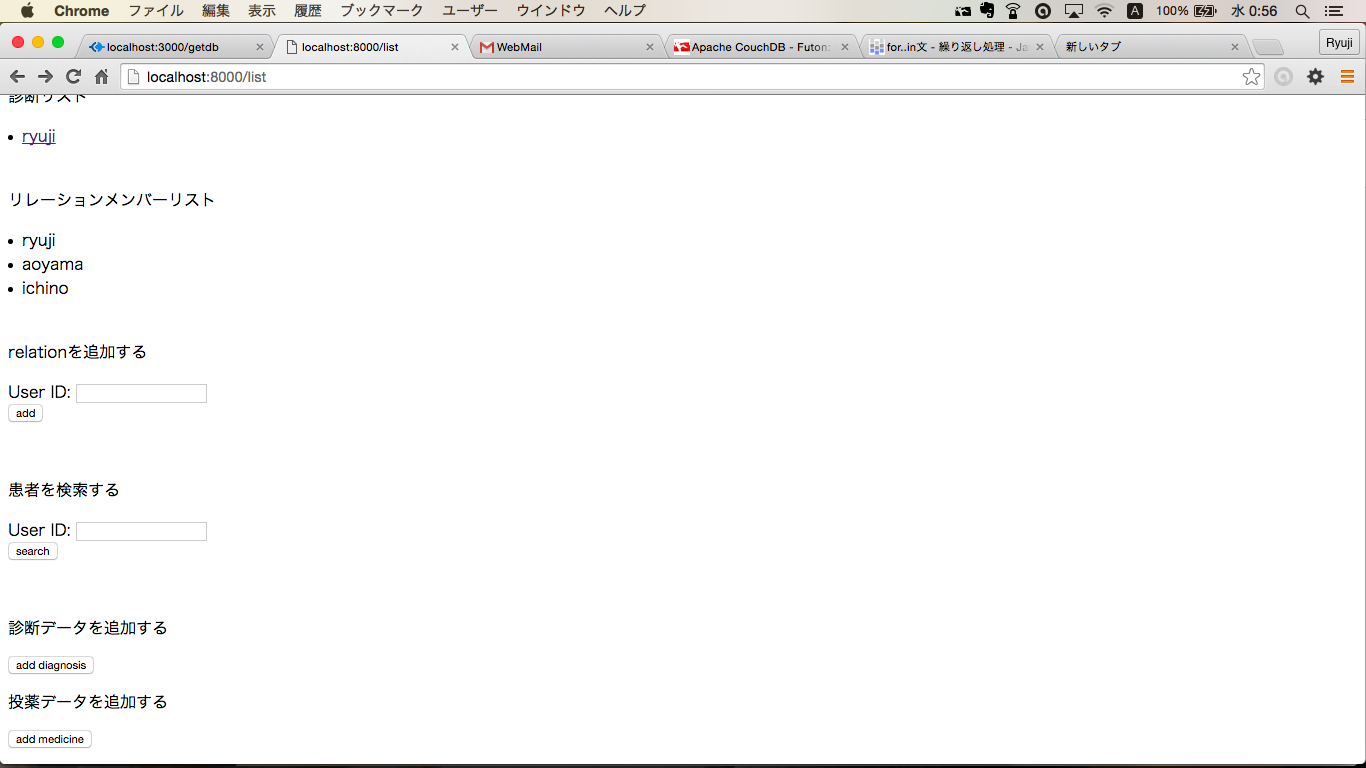
\includegraphics[width=5cm, bb=0 0 645 790]{./gazou/DjangoFileio.png} %よこたて
  		\end{center}
  		\caption{データ入力}
  		\label{DjangoFileio}
  	\end{figure}

  \subsubsection{データ閲覧}
    \begin{figure}[htbp]
      \begin{center}
        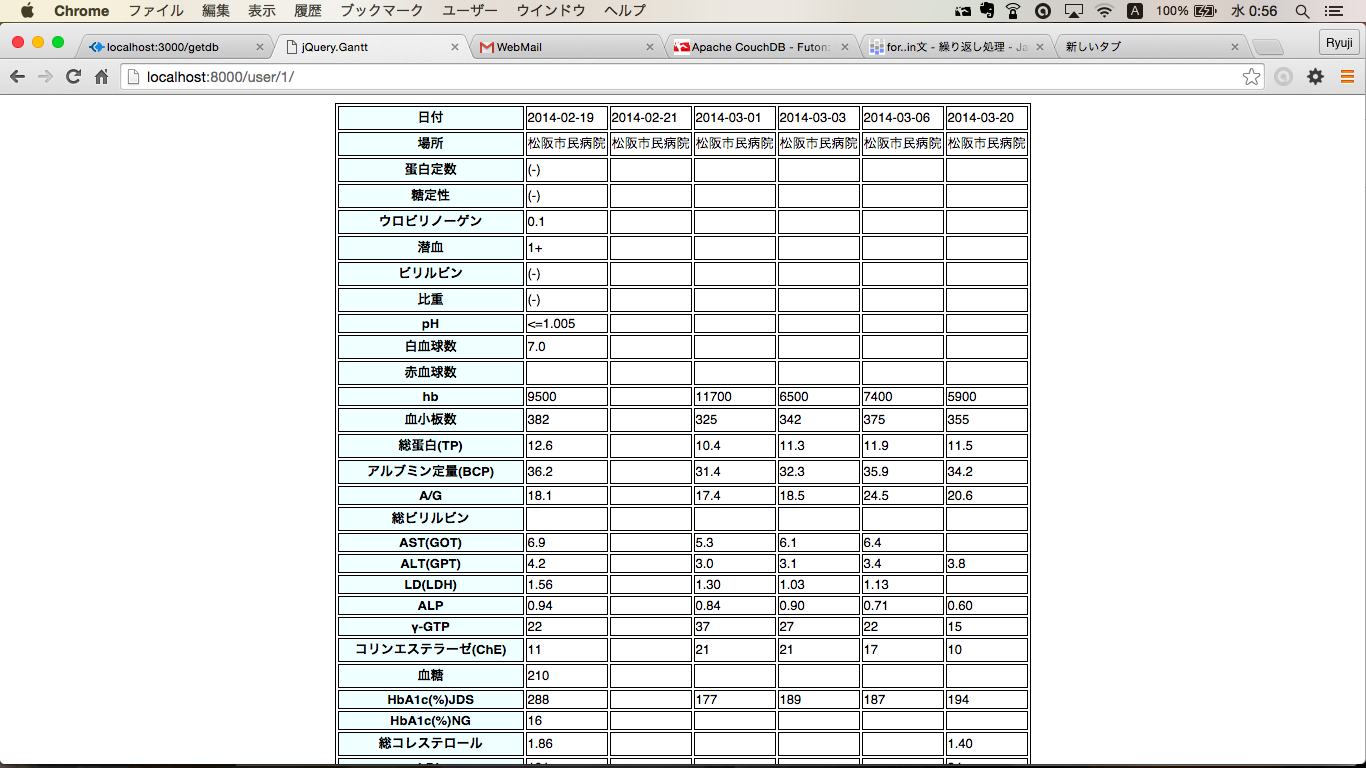
\includegraphics[width=5cm, bb=0 0 645 790]{./gazou/DjangoTable.png} %よこたて
      \end{center}
      \caption{表によるデータ閲覧}
      \label{DjangoTable}
    \end{figure}

    \begin{figure}[htbp]
      \begin{center}
        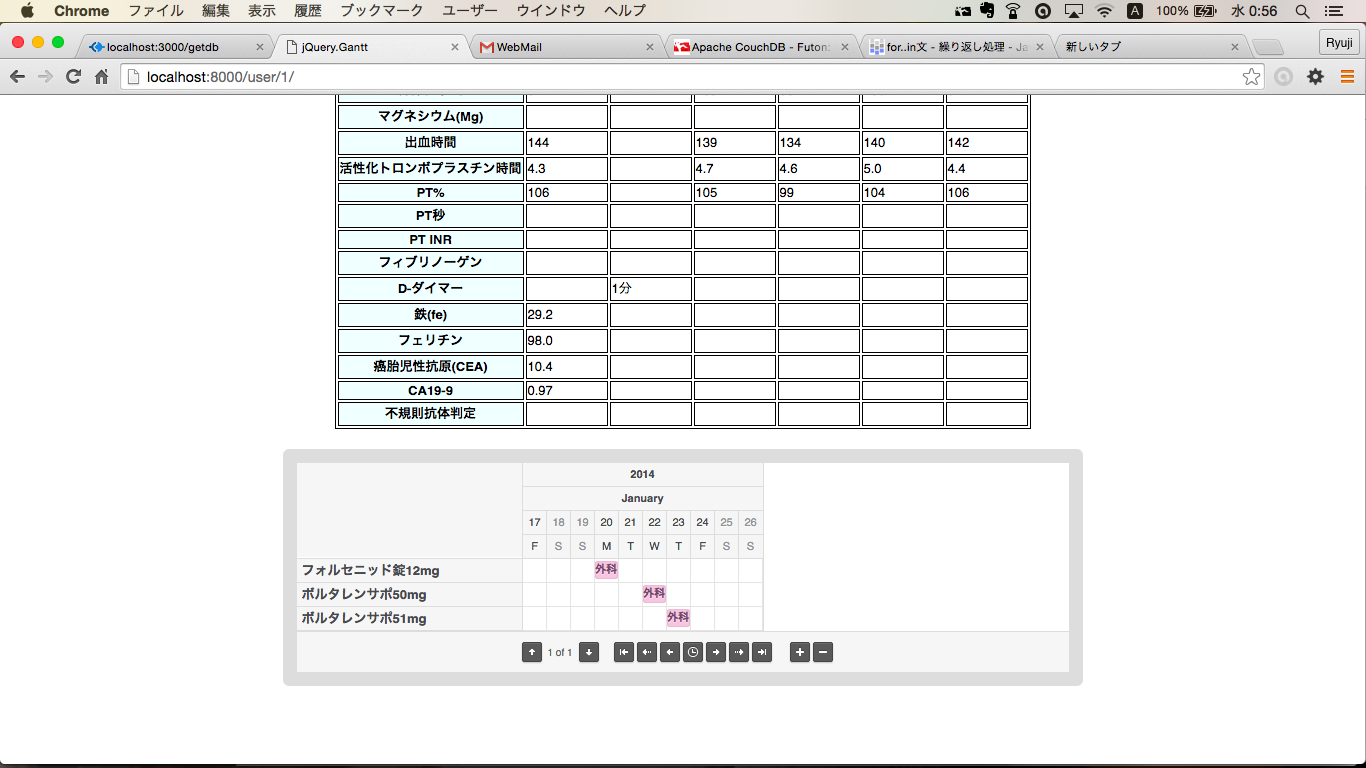
\includegraphics[width=5cm, bb=0 0 645 790]{./gazou/DjangoGantt.png} %よこたて
      \end{center}
      \caption{ガントチャートによるデータ閲覧}
      \label{DjangoGantt}
    \end{figure}

  \subsubsection{権限の付与}


\subsection{SQL版の課題とフィードバック}

  開発アプリのデモンストレーションによって得た医療関係者からの意見の中で
  研究課題として任意の検査項目の抽出が挙げられる.

  他の意見はインターフェース寄りの要望が多かった.
  例えば,表によるデータの表示に対するフィードバックとして,

  \begin{itemize}
    \item 任意の検査項目にハイライトをつけてほしい
  \end{itemize}


  今後需要があるであろうバイタルデータの活用に向けて,
  NoSQLを用いたアプリ開発を行う.

  ドキュメントの数だけSQLデータベースのテーブルを用意する必要がある.
  データを検索する際にはjoinしてから.
  比べてNoSQLならガンガン入れて,
  データを出すときにだけKeyの関連づけをすればよい.
  NoSQLならSQLに比べてテーブルを用意する分の
  コストがはぶけてる(と言えるかな).
